\chapter{Overall Description}
\label{cha:desc}

\section{Product perspective}
\label{sec:productperspective}
The application will be available through web and mobile devices, keeping the same look and elements along the various implementations.
The user experience through the application should be easy and natural.
The application developed allow the time slotting ahead the upcoming events so that the user can have a full view of the day with a prediction of the travel time between the appointments if they are in different locations.
The event can regard working or personal aspects, and in any case, the application will notify or suggest a different mean of transport based on the weather conditions or strikes of the public transport.


\section{Product functions}
\label{sec:productfunctions}
The application allows you to schedule events, choose which mean of transport and get warned in case of overlapping events
On top of the time allocation, there will be a cost estimation provided when possible. 
This will allow the user to filter the possible mean of transport based on carbon footprint emission, price impact and time.

A User can:
\begin{itemize}
\item Create an event:
\begin{itemize}
\item Modify an event
\item Invite other users to their events
\end{itemize}
\item Receive help to reach the location of the next event
\begin{itemize}
\item Buying tickets for a mean of transport that require tickets
\item Providing navigation for reaching the spot 
\end{itemize}
\end{itemize}
\begin{itemize}
\item Get notified
\begin{itemize}
\item Upcoming events
\item Free space
\end{itemize}
\end{itemize}


\begin{figure}[H]
  \centerline{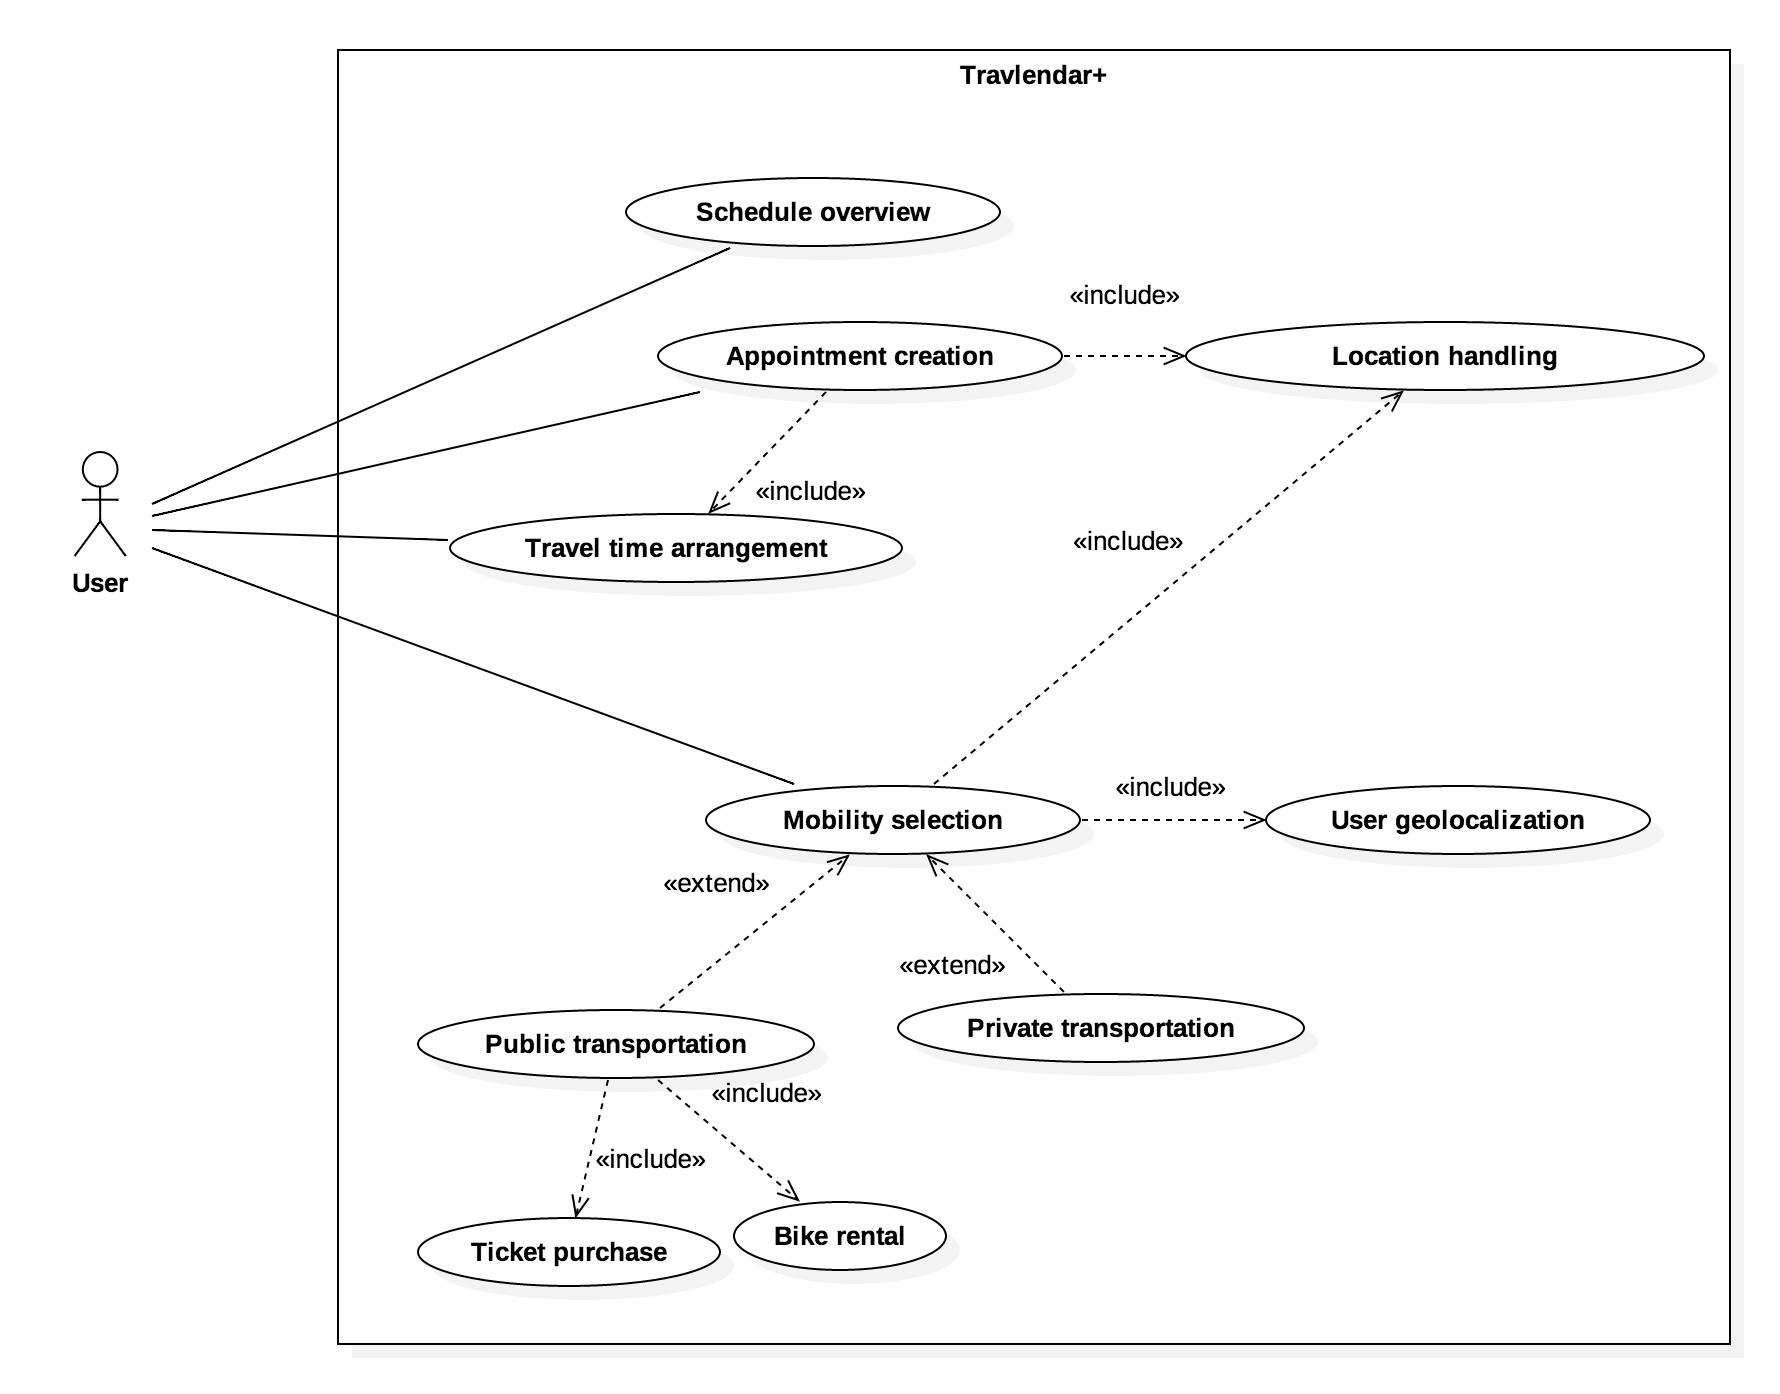
\psfig{file=diagrams/UseCaseDiagram.png,width=\textwidth} }
  \caption{Comprehensive use case diagram.}   
\end{figure}

\begin{figure}[H]
 \centerline{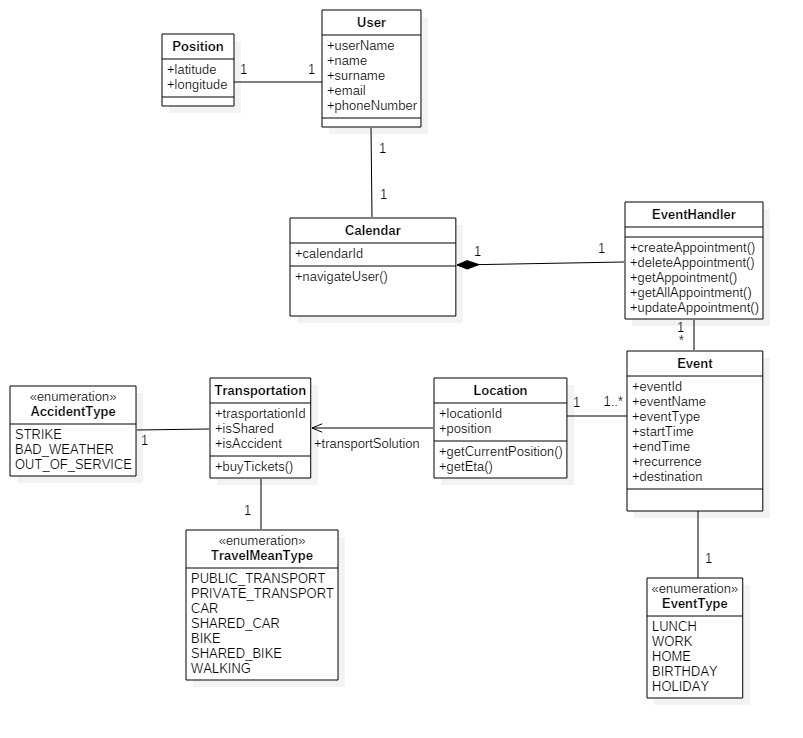
\psfig{file=diagrams/ClassDiagram.png,width=\textwidth} }
 \caption{Comprehensive class diagram.}  
\end{figure}

\section{User characteristics}
\label{sec:usercharacteristics}
\begin{description}
\item There is one type of user, which can be interfaced with other users in case of shared meetings.
\item Instead, the users that receive the invite will have read-only permissions.
\end{description}

\section{Assumptions, dependencies and constraints}
\label{sec:assumpdepenconst}

\paragraph{Text assumptions}
\begin{itemize}
\item The user will be able to schedule only future events, with the option to recur on a daily, weekly or monthly basis.
\item The working events can only be scheduled within the working hours, reserving at least 30 minutes for the lunch break.
\end{itemize}

\paragraph{Domain assumptions}
\begin{itemize}
\item {[D1]} Two events can be overlapping but cannot start and end at the same time (for instance, one event occurs throughout the day).
\item {[D2]} The event that overlap the other cannot have an end time previous the event started before.
\item {[D3]} The event located within the same location have no mobility option (navigation/buying tickets).
\item {[D4]} Working events can be scheduled within the working hours.
\item {[D5]} The user have to configure his habits (working hours, owning a car/bike) at the first use of the application.
\end{itemize}

\paragraph{Dependencies}
\begin{description}
\item We will depend on Google Maps API’s to get the estimation of the time to get the distance between 2 locations. 
We will access the Google Maps Distance Matrix API through an HTTP interface, with requests constructed as a URL string, using origins and destinations.
\item During the process to buy the tickets of the public transport system we will redirect the user to the provider of the service, or when allowed the user will be deep-linked to the desired application.
\end{description}


\paragraph{Constraints}
\begin{description}
\item To ensure enough level of privacy and avoid security breaches, every request containing the user’s position will be handled within an HTTPS connection.
\end{description}
